% !TeX root = RJwrapper.tex
\title{Splitting It Up: The \pkg{spduration} Split-Population Duration
Regression Package for Time-varying Covariates}
\author{by Andreas Beger, Daniel W. Hill, Jr., Nils. W. Metternich, Shahryar Minhas, and Michael D. Ward}

\maketitle

\abstract{
We present an implementation of split-population duration regression in
the \CRANpkg{spduration} \citep{beger2016spduration} package for {\sf R} \citep{rstats2016} that allows for time-varying covariates. The statistical model accounts for units that are immune to a
certain outcome and not part of the duration process the researcher is
primarily interested in. We provide insights that if immune units exist,
we can significantly increase the predictive performance compared to
standard duration models. The package includes estimation and several
post-estimation methods for split-population Weibull and Loglogistic
models. We provide an empirical application to data on military
coups.
}

\section{Introduction}

Duration models are an important class of statistical estimators that
take into account the duration dependency of specific outcomes. A
prominent example is that the risk of dying depends on the age of an
individual. Newborns are at a greater risk of dying, but as they grow
older this risk quickly declines and then gradually starts to increase
again after the age of 9-10. While individual behavior (smoking,
exercising, diet) and structural factors (health care, health
regulations, urban vs rural) can increase or decrease the probability of
dying over time, the underlying risk is time dependent and impacts on
all individuals.

However, there are conditions under which not all individuals have the
same underlying risk to experience a specific outcome and might not even
be at risk at all. Consider the risk of acquiring a viral infection like
the common flu. Let us initially assume that everyone is at risk of
infection, and individual behavior (e.g., good hygiene) and structural
factors (e.g., workplace) determine whether individuals catch the flu.
Under these assumptions a standard duration model should provide us with
efficient estimates of how different behavioral and structural factors
impact on the general baseline risk. But, there might be individuals
that are immune to the flu in the overall population--because they
received vaccination, had the specific flu virus in the past, or have
some other characteristic that makes it impossible for them to attract
the disease. In this instance we have two underlying populations: an at
risk population and an immune one. If the immune population is
relatively large, estimates using a standard duration model will be
biased and predictions inaccurate.

\section{Immune populations and inference of duration
processes}

Regular duration models, where baseline risk is modeled by some
distribution of time, were originally developed in health and
demographic research and grew naturally from life tables and survival
records for medical patients. Basic formulations of such models, like
the parametric exponential or Weibull regressions or semi-parametric Cox
regression, implicitly assume that all subjects or units under
observation, including right-censored observations, will eventually
experience the event of interest. This assumption may be violated in
many substantive areas and empirical applications, where a
sub-population of units or individuals will never experience an event,
and thus are effectively ``cured''.

The insight that populations might be split in regard to their baseline
risk has been formulated as early as 1949 by \citet{boag1949maximum} and \citet{berkson1952survival}, who were researching survival rates in cancer patients. In
their application some fraction of patients survived because their
cancer was cured, while others relapsed after apparent remission due to
levels of disease below detectable thresholds. The development of
duration methods in health and medicine has also shaped the terminology
conventionally used for such models. For example, split-population
duration models are also referred to as cure rate models. Similarly, the
basic concepts like survival and failure rates reference the survival of
humans.

Yet the intuition underlying split-population duration models has led to
applications in a broad range of subject areas outside demographics and
medicine. In an early and foundational application that reached beyond
medicine, \citet{schmidt1989predicting} examined criminal recidivism using
data on close to 10,000 prisoners from the North Carolina prison system
in the late 1970's and early 1980's to identify factors that influence
whether a criminal relapses at all, and if so which factors are related
to the amount of time between prison stints. This work already includes
a full formulation of a model with independent covariates for both the
duration equation and the risk or cure equation, although only with
subject-specific covariates rather than time-varying covariates for
multiple data points per individual.

In a complementary set of research from public health, \citet{douglas1994hazard} use data from the United States to model the age at
which individuals began to smoke, and \citet{forster2001role} examine
the impact of tobacco taxes on smoking and quitting decisions. \citet{deyoung2003failure}, an economist, models the failure of new commercial banks in the
US during the 1980's. \citet{svolik2008authoritarian} uses a split-population duration
framework to examine whether democratic regimes persist or revert to
authoritarianism, and when. Building on this effort, split-population
duration models have also been used, along with other models, to produce
regular predictions for five different forms of political conflict for
the Integrated Crisis and Early Warning System (ICEWS) project \citep{ward2013learning} and to model irregular leadership changes for the Political
Instability Task Force \citep[PITF;][]{beger2014ensemble}.

\section{Model development}

Conventional duration models assume that all subjects will eventually
fail, die, or experience a specific outcome. The likelihood for a data
point with survival time \(t\) is thus the failure rate \(f(t)\) at that
time or the probability of survival beyond \(t\), \(S(t)\), depending on
whether the subject has already experienced the event (\(\delta_i\)) or
is right-censored (\(1-\delta_i\)):

\begin{eqnarray}
\mathcal{L} = \prod_{i=1}^N  \left( f(t_i)\right)^{\delta_i} \times \left( S(t_i) \right)^{1-\delta_i}
\end{eqnarray}

The major modeling question in this setting, which we will return to
below, is the choice of a function form (e.g., exponential, Weibull, or
log-logistic) describing the underlying hazard rate
\(h(t) = \frac{f(t)}{S(t)}\) over time.

The cumulative failure rate (\(F(t) = 1 - S(t)\)) over time converges to
1, meaning all subjects fail eventually. In the examples of applied
research discussed above this assumption is untenable. Some cancer
patients are cured after treatment, most young people never become
regular smokers, and many states will not experience the kind of
violence that persists in other parts of the world. The presence of a
large sub-population which is not at risk for an event, will in practice
inflate estimates of the survival fraction, and reduce hazard estimates
for all subjects. This is the case because the underlying risk is
estimated based on subjects that genuinely will fail and those that are
cured. Hence, such a model will over predict the hazard for subjects
that are not at risk (cured), and under predict for those who are at
risk of eventually experiencing the event of interest.

We can incorporate the presence of a sub-population, where we label the
subpopulation at risk with \(\pi\), by rewriting the likelihood
as:\footnote{Usual presentation of the split-population duration framework in medical contexts focus on the ``cured'' subpopulation. In our applications events are typically rare and it thus is easier to emphasize the ``risk'' subpopulation. As risk $= 1 - $ cured, this difference is trivial.}

\begin{align}
\mathcal{L}\{\theta|(t_{1}, \dots, t_{n})\} &= \prod_{i=1}^{N} \left(\pi_i f(t_i)\right)^{\delta_i} \times  \left((1-\pi_i) + \pi_i S(t_i)\right)^{1-\delta_i}
\end{align}

Crucially, this split-population framework is primarily useful in
contexts where sub-populations are not clearly or easily identifiable.
For example, there is a clear sub-population in a model of the age at
first pregnancy for humans---men---which researchers can easily identify
and exclude from their data. Less clear are answers to questions such as
whether a cancer patient is cured or not cured given that they have no
visible signs of cancer following treatment or have hit the 5-year
disease free survival mark. In such situations split-population models
provide a way to infer sub-populations in a probabilistic fashion.

Early efforts focused only on the cure rate (\(1 - \pi\)) and treated it
as a constant, but we can model membership in the subpopulation with its
own covariates through a logistic link function:

\begin{align}
\pi_i &= \frac{1}{1 + e^{-z_i \gamma}}
\end{align}

Where \(z_i\) is a vector of covariates for a subject at a given time.
For interpretation, it is important to note that with time-varying
covariates, the risk (or cured) estimate for a subject is particular to
a given time point rather than constant over all time periods in the
spell.\footnote{We use ``spell'' to designate all time periods observed for a subject up to the failure time. Subjects can theoretically have multiple spells, e.g., cancer patients who go into remission and relapse more than once, or states that experience multiple civil wars over their history.}
Depending on the covariates, the risk estimate for a subject can thus
fluctuate over time. To ease interpretation, it might be convenient to
restrict covariates in the logit risk model to slow-moving, stable
covariates in order to produce stable risk estimates for subjects.

The last component to complete the likelihood is the choice of a
distribution for the shape of the hazard rate. The \CRANpkg{spduration}
package implements two hazard rate shapes, Weibull and log-logistic:

\begin{eqnarray*}
\textrm{Weibull} \\
 f(t) & = & \alpha \lambda (\lambda t)^{\alpha - 1} e^{-(\lambda t)^\alpha} \\
  S(t) & = & e^{ -(\lambda t )^\alpha } \\
 h(t) & = & \alpha \lambda (\lambda t)^{\alpha-1} \\
\textrm{Log-logistic} \\
 f(t) & = & \frac{ \alpha \lambda (\lambda t)^{\alpha-1} }{ (1 + (\lambda t)^\alpha)^2 } \\
 S(t) & = & \frac{1}{ 1+  (\lambda t)^\alpha }  \\
 h(t) & = & \frac{ \alpha \lambda (\lambda t)^{\alpha-1} }{ 1+  (\lambda t)^\alpha }
\end{eqnarray*}

Where \(\lambda = e^{-x_i\beta}\) is a parameter of covariates. The
Weibull density allows for hazard rates that are increasing, constant,
or decreasing over survival time, while the log-logistic density also
can fit rates that have a peak at a particular survival time.

Given the density distribution, the main quantity of interest is the
conditional hazard \(h(t, \pi)\), where both the risk/cure probabilities
and hazard are conditional on survival to time \(t\):

\begin{eqnarray}
h(t, \pi) = \frac{f(t, \pi)}{S(t, \pi)} & = & \frac{ \pi(t) \times f(t) }{ (1-\pi(t)) + \pi(t) \times S(t) } \\
 \pi(t) & = & \frac{ 1-\pi }{ S(t) + (1-\pi) (1 - S(t)) }
\end{eqnarray}

For a given unconditional risk rate \(\pi\), the probability that a
subject with survival time \(t\) is in the risk set decreases over time,
because an increasing number of surviving cases consist of immune or
cured (\(1-\pi\)) cases that will never fail. In the hazard rate, the
failure rate in the numerator is conditional on the probability that a
case is in the risk set, given survival up to time \(t\), and the
numerator is an adjusted survivor function that accounts for the
fraction of cured cases by time \(t\), which is \(1-\pi(t)\).

\section{Fit a split-population model on coups
data}

In order to illustrate the package functionality, we examine a model of
coups d`etat in \citet{belkin2003toward}. Belkin and Schofer's paper
lends itself to re-analysis with a split-population duration model
because they explicitly distinguish long-term structural risk factors
for coups from more short-term triggering causes that can explain the
timing of a coup in an at-risk regime. They argue that many countries
never experience coups because coups are effectively impossible due to
structural factors, while others that never experience coups are
nevertheless at risk due to a different configuration of those same
factors. Using language which fits nicely with the class of models
described above, they write ``{[}t{]}riggers are not the source of the
original risk, and in the absence of structural causes, the presence of
triggering factors alone cannot lead to a coup. Hence, triggers should
not be equated with coup risk. Rather, they are factors that may
determine the exact timing of a coup in regimes that suffer from high
coup risk'' (Belkin and Schofer 2003, 598).

For their empirical test Belkin and Schofer develop a measure of
``structural coup risk'' which incorporates factors such as the strength
of democratic institutions and civil society, and a recent history of
successful coups. However, they implement a logistic regression model,
which does not capture the process as described in their quote above.
This is because the logistic regression model assumes that all
observations are at risk for a coup (i.e., the probability of a coup is
non-zero for all observations). Since their structural coup risk
indicator is developed precisely to distinguish between at risk and
``immune'' cases, the split-population model allows one to examine
whether the indicator effectively does so.

We begin by loading the package and the Belkin and Schofer replication
data, and formatting the data to add several variables needed by the
split-population duration model.

\begin{example}
  library("spduration")
  data(bscoup)
  ?bscoup
  head(bscoup[, 1:5])
    countryid  year  couprisk recentcoups rwar
  1       909  1960 0.2200166           0    0
  2       909  1961 0.2200166           0    0
  3       909  1962 0.2200166           0    0
  4       909  1963 0.2200166           0    0
  5       909  1964 2.5702426           1    0
  6       909  1965 2.5702426           2    0
\end{example}

The data are documented in \samp{?bscoup}, which also gives a reference to the source citation. It consists of a little more than 5,000 observations of 162 countries from 1960 to 2000. Each row corresponds to a country $c$ in year $t$. Excluding the country and year identifiers, the data include 12 variables, including a binary indicator for successful coups. 

\begin{example}
  str(bscoup)
  'data.frame':	5463 obs. of  14 variables:
  $ countryid  : num  909 909 909 909 909 909 909 920 920 920 ...
  $ year       : num  1960 1961 1962 1963 1964 ...
  $ couprisk   : num  0.22 0.22 0.22 0.22 2.57 ...
  $ recentcoups: num  0 0 0 0 1 2 4 0 0 0 ...
  $ rwar       : num  0 0 0 0 0 0 1 0 0 0 ...
  $ milreg     : num  0 0 0 1 0 1 1 0 0 0 ...
  $ wealth     : num  NA NA NA NA NA ...
  $ instab     : num  4 2 9 9 12 13 12 NA 0 4 ...
  $ coup       : Factor w/ 2 levels "no","yes": 1 1 1 2 2 2 1 1 1 1 ...
  $ africa     : num  0 0 0 0 0 0 0 0 0 0 ...
  $ eurnam     : num  0 0 0 0 0 0 0 1 1 1 ...
  $ samerica   : num  0 0 0 0 0 0 0 0 0 0 ...
  $ camerica   : num  0 0 0 0 0 0 0 0 0 0 ...
  $ regconf    : num  0 0 0 0.019 0.019 ...
  - attr(*, "datalabel")= chr ""
  - attr(*, "time.stamp")= chr "30 Jul 2003 12:15"
  - attr(*, "formats")= chr  "%9.0g" "%9.0g" "%9.0g" "%9.0g" ...
  - attr(*, "types")= int  102 102 102 102 102 102 102 102 102 102 ...
  - attr(*, "val.labels")= chr  "" "" "" "" ...
  - attr(*, "var.labels")= chr  "country code .pr89" "year coded" "" "" ...
  - attr(*, "version")= int 7
  - attr(*, "label.table")=List of 1
  ..$ hadcoup: Named int  0 1
  .. ..- attr(*, "names")= chr  "no" "yes"
  bscoup$coup <- ifelse(bscoup$coup == "yes", 1, 0)
  table(bscoup$coup)
  0    1
  5173  290 
\end{example}

Altogether the data include 290 coups, which makes for a positive rate of slightly more than 5\% of all observations. 

Before we can estimate a split-population duration model with the data, we need to add several variables that capture the survival characteristics of the data.

\begin{example}
  bscoup <- add_duration(bscoup, "coup", unitID = "countryid", 
  +    tID = "year", freq = "year", ongoing = FALSE)
  Warning message:
  In attempt_date(data[, tID], freq) :
  Converting to 'Date' class with yyyy-06-30
\end{example}

The \code{add\_duration} function takes as input a data frame with a
binary response variable--\code{coup}--that measures the occurrence of the
event, or failure, recorded over discrete time periods. We assume that
the data frame is in a cross-sectional time-series format that consists
of multiple observations over time for a number of subjects, in our case
countries.

Within the framework of duration modeling, these data conceptually
consist of ``spells'', which are repeated observations of a unit from
the time they enter the data (left-censoring) or after they experienced
the event of interest, until the next event or the end of observation
(right censoring). Table \ref{tab-ex} shows how a single country could
have two spells during the observation period. Observations for Portugal
make up two spells, one that begins in 1960, when our data start, to a
coup event in 1975, when a second spell starts and continues until
either the next coup or the data end. Canada on the other hand
experienced no coups and so observations for that country from 1960 to
2000 make up one spell.

\begin{table}
\begin{center}
\begin{tabular}{lrrrrr} \toprule
Country & Year & Coup & Spell ID & Duration \\ \midrule
Portugal & 1960 & 0 & 1 & 1  \\ 
\ldots & \ldots & 0 & 1 & \ldots \\
\ldots & 1975 & 1 & 1 & 16 \\ \midrule
Portugal & 1976 & 0 & 2 & 1 \\
\ldots & \ldots & 0 & 2 & \ldots \\
\ldots & 2000 & 0 & 2 & 20  \\ \midrule
Canada & 1960 & 0 & 3 & 1 \\
\ldots & \ldots & 0 & 3 & \ldots \\ 
\ldots & 2000 & 0 & 3 & 41 \\ \bottomrule
\end{tabular}
\end{center}
\caption{Example data frame with select duration variables.} \label{tab-ex}
\end{table}

The \code{add\_duration} functions identifies spells in the data and
returns the data frame with several additional variables needed for
estimation. The most important among these are a counter of elapsed time
in a spell, \code{duration}. It also codes that a spell was at risk
(\code{atrisk==1}) if it ended in a failure event, and not at risk
otherwise. These are then used as response variables for the formula in
the \code{spdur} function.

Though the data used in this example are recorded annually, the function
supports annual, monthly, or daily data and will try to convert the
\code{tID} input to class \code{Date} given the provided argument in
\code{freq}, as indicated by the warning it returned in the example above. This 
can be avoided by converting any numeric dates to {\sf R} \code{Date}s first.

Another important question is how to handle consecutive 1's
in the response variable provided. This is controlled with the
\code{ongoing} argument. In some cases like civil war occurrence, the
\emph{y} variable records all years during which a country experienced a
civil war. Here \code{ongoing} should be set to true so that the models
try to predict the onset of the civil war, but disregard ongoing
conflicts (\code{failure} is set to \code{NA} for these cases, dropping
them from analysis). With ongoing set to false, successive 1's in
\emph{y} are treated as distinct and new failures, and kept in the
analysis. This makes sense for discrete, short-term events like coups.
Countries can experience distinct coups in successive years.

The \code{spdur} function is the primary function in the package and
produces a regression model object of class \code{spdur} which can then
be used with further methods. We begin by fitting first a Weibull and
then a log-logistic split-population duration model using the coups
data, including the measure of coup risk in the logit (risk) equation.

\begin{example}
  weib_model <- spdur(
  +    duration ~ milreg + instab + regconf,
  +    atrisk ~ couprisk + wealth + milreg + rwar + regconf + samerica + 
  +      camerica,
  +    data = bscoup, silent = TRUE)

  loglog_model <- spdur(
  +    duration ~ milreg + instab + regconf,
  +    atrisk ~ couprisk + wealth + milreg + rwar + regconf + samerica + 
  +      camerica,
  +    data = bscoup, distr = "loglog", silent = TRUE)
\end{example}

Using the \code{summary} function on either model object will produce
standard output showing the model formula, estimates for the duration
and risk equations, and test statistics with \(p\)-values. These can be
exported by calling \code{xtable}\citep[see][]{dahl2016xtable} directly on the \code{spdur} object to
produce Table 2.

\begin{example}
  library("xtable")
  tbl <- xtable(loglog_model, caption = "Coup model with log-logistic hazard",
  +    label = "loglog_table")
  print(tbl, caption.placement = "top", comment = FALSE, 
  +    include.rownames = FALSE)
\end{example}

\begin{table}[ht]
\centering
\begin{tabular}{lrrrr}
  \hline
Parameter & Estimate & Std. Error & t value & Pr($>$$|$t$|$) \\ 
  \hline
Dur\_(Intercept) & 2.40 & 0.21 & 11.43 & 0.00 \\ 
  Dur\_milreg & $-$1.13 & 0.21 & $-$5.46 & 0.00 \\ 
  Dur\_instab & $-$0.09 & 0.02 & $-$4.79 & 0.00 \\ 
  Dur\_regconf & $-$2.52 & 2.16 & $-$1.16 & 0.24 \\ 
  log(alpha) & $-$0.45 & 0.06 & $-$7.09 & 0.00 \\ 
  Risk\_(Intercept) & 2.93 & 1.87 & 1.57 & 0.12 \\ 
  Risk\_couprisk & 0.59 & 0.32 & 1.82 & 0.07 \\ 
  Risk\_wealth & $-$0.36 & 0.28 & $-$1.29 & 0.20 \\ 
  Risk\_milreg & 10.82 & 9.31 & 1.16 & 0.25 \\ 
  Risk\_rwar & $-$0.52 & 0.94 & $-$0.56 & 0.58 \\ 
  Risk\_regconf & $-$5.43 & 5.62 & $-$0.97 & 0.33 \\ 
  Risk\_samerica & 2.09 & 1.45 & 1.45 & 0.15 \\ 
  Risk\_camerica & $-$0.39 & 0.73 & $-$0.53 & 0.59 \\ 
   \hline
\end{tabular}
\caption{Coup model with log-logistic hazard.} 
\label{loglog_table}
\end{table}

Table~\ref{loglog_table} shows estimates from the duration equation,
beginning with the intercept, and then estimates from the risk equation.
The duration component of the model is in accelerated failure time
format and the coefficient estimates are on the log of expected time to
failure. The negative coefficient for military regimes for example means
that the expected time to a coup is shorter in military regimes than
non-military regimes, holding all other factors constant. In the risk
equation, positive coefficients mean higher risk of coup. Thus, military
regimes have a higher risk of experiencing a coup.

One may also use the \code{AIC} and \code{BIC} function to calculate the
information criterion statistics for \code{spdur} objects. In our
example, both models are close enough in both statistics to be
indistinguishable, so we will continue to focus on the log-logistic
form.

\begin{example}
  matrix(c(
  +    AIC(weib_model), AIC(loglog_model), BIC(weib_model), BIC(loglog_model)
  +    ), ncol = 2, dimnames = list(c("Weibull", "Loglog"), c("AIC", "BIC")))
               AIC      BIC
  Weibull 1329.908 1348.972
  Loglog  1331.214 1350.278
\end{example}

The package includes two types of plots that show the estimated hazard rates and 
predictive performance, respectively. The hazard rates can be plotted by either 
calling \code{plot\_hazard} directly, or with \code{plot(x, type = "hazard")}, on
a fitted \code{spdur} object. It will produce a plot of the conditional hazard, which is the probability of survival conditional on the covariates in the risk and
duration equations, and conditional on survival up to time \(t\), when holding
all covariates at their sample means. The
function calculates the average hazard rate as well as 90\% confidence
intervals, which are produced by simulating values from the estimated
sampling distributions of the model parameters. 

\begin{example}
  plot(weib_model,   type="hazard", main="Weibull")
  plot(loglog_model, type="hazard", main="Loglog")
\end{example}

\begin{figure}
\begin{center}
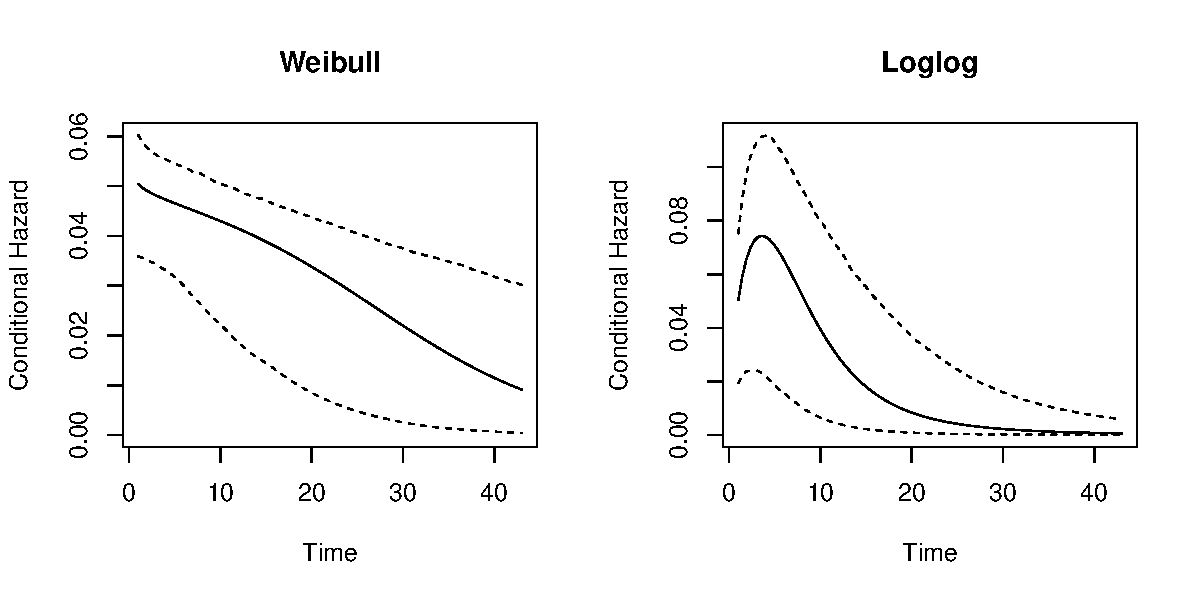
\includegraphics[width=0.8\textwidth]{graphics/hazard-rates.pdf}
\caption{Hazard rate plots for the Weibull and Loglogistic coup models.}
\label{hazard-ex}
\end{center}
\end{figure}

By default the \code{plot\_hazard} function
uses the mean values of the covariates during the simulations, but users
can choose specific covariate values by entering them as vectors in the
arguments \code{xvals} and \code{zvals}, which correspond to the
covariates in the duration and risk equations, respectively. The command
below creates the graph A in Figure \ref{hazard-ex}.

\begin{example}
  plot_hazard(loglog_model, main = "A")
\end{example}

\begin{figure}
\begin{center}
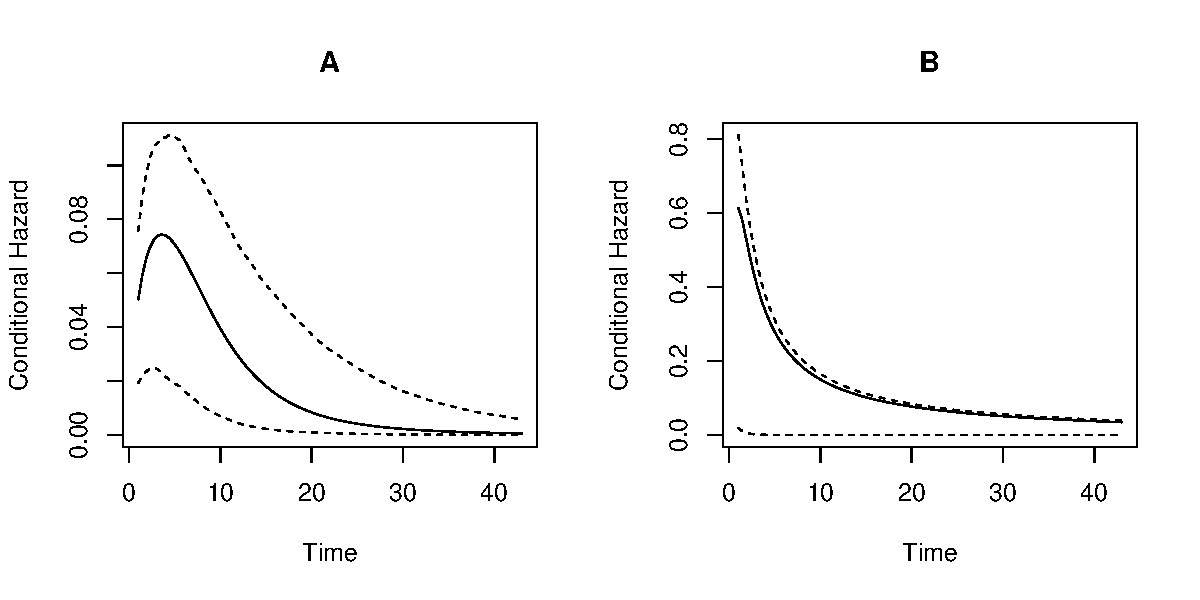
\includegraphics[width=0.8\textwidth]{graphics/hazard-ex.pdf}
\caption{Plots of the hazard rate for the log-logistic model of coups. Graph A uses the default mean values for covariates, while graph B uses user-specified variable values for a high-risk military regime.}
\label{hazard-ex}
\end{center}
\end{figure}

As mean values are maybe not that interesting, we can also generate
scenarios by entering values manually. The values are used in the same
order that variables are specified in the equations used to estimate the
models, which also corresponds to the order of variables in Table 2.
Note the inclusion of an intercept term. This produces plot B in Figure
\ref{hazard-ex}

\begin{example}
  plot_hazard(loglog_model, xvals = c(1, 1, 10, 0.05), 
  +    zvals = c(1, 7, 8.64, 1, 1, 0.05, 0, 0), main = "B")
\end{example}

While \code{plot(x, type = "hazard")} will produce a hazard rate plot, without a type argument,
\code{plot.spdur} will produce a separation plot. Separation plots are a graphical
display for evaluating model predictions \citep{greenhill2011separation}. The code below produces Figure \ref{insamp}.

\begin{example}
  plot(weib_model)
  plot(loglog_model)
\end{example}

\begin{figure}
\begin{center}
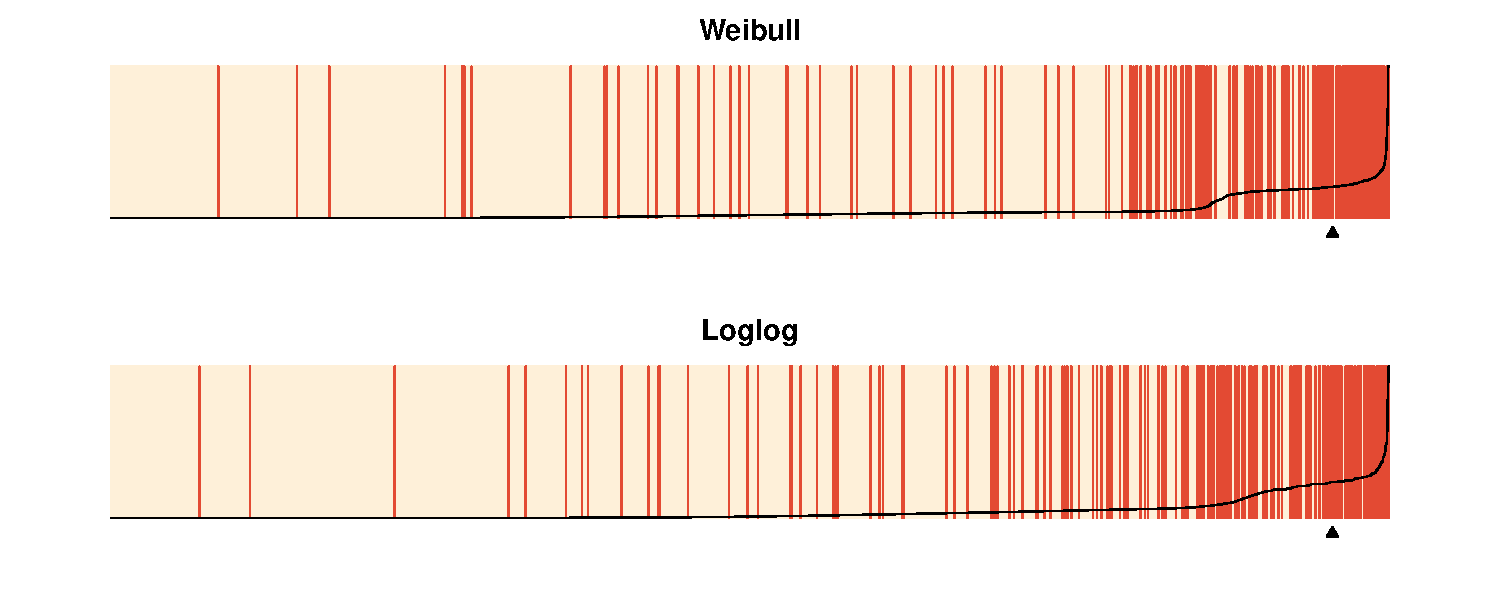
\includegraphics[width=0.8\textwidth]{graphics/sepplots.pdf}
\caption{In-sample separation plots of Weibull and log-logistic model conditional hazard predictions.}
\label{insamp}
\end{center}
\end{figure}

The option \code{endSpellOnly} is set to \code{FALSE} so that every
observation, not only those at the end of a spell, is used in the plot.
By default the \code{plot} function will calculate the conditional
hazard for each observation. The separation plot sorts observations from
left to right according to the predicted probability assigned by the
model (higher values to the right), and shows each event/failure as red
line, with non-events shown in beige. This makes it easy to see whether
the model is assigning high probabilities of failure to actual cases of
failure, and low probabilities to non-failures.

Underlying both plotting functions is the \code{predict} function, which
can be used on an object of class \code{spdur} to generate several kinds
of predictions, including the probability that an observation is
``at-risk'' and the probability of failure for a given time period.

\subsection{Out-of-sample testing}

Finally, we demonstrate how to evaluate a model's out of sample
predictions. We will use data from 1996 onwards as the test set, and
prior data for training purposes. The \code{add\_duration} function
retrospectively codes the risk variable based on how a spell ended, and
we therefore need to take care in how we add the duration variables for
each data set. For the training data we need to subset the training set
first, so that coups in the tests set don't influence the risk coding in
the training data.

\begin{example}
  data(bscoup)
  bscoup$coup <- ifelse(bscoup$coup == "yes", 1, 0)
  coup_train <- bscoup[bscoup$year < 1996, ]
  coup_train <- add_duration(coup_train, "coup", unitID = "countryid", 
  +    tID = "year", freq = "year", ongoing = FALSE)
\end{example}

For the test set it is recommended to add the duration variables and \textit{then} subset the test set. Since the test set is later in time than the training set we do not have to worry about contamination of the risk coding, but if we subset the data before building the duration variables we will start all duration counters at 1996, when in fact we can safely use the previous historic coup information. To do this we need to build the duration variables first:

\begin{example}
  coup_test  <- add_duration(bscoup, "coup", unitID = "countryid", 
  +    tID = "year", freq = "year", ongoing = FALSE)
  coup_test  <- coup_test[coup_test$year >= 1996, ]
\end{example}

Now we can fit new models using the training data, and calculate
predictions from these models for the test data, using
\code{predict(..., newdata = coup\_test)}.

\begin{example}
  weib_model2   <- spdur(
  +    duration ~ milreg + instab + regconf,
  +    atrisk ~ couprisk + wealth + milreg + rwar + regconf + samerica + 
  +      camerica,
  +    data = coup_train, silent = TRUE)

  loglog_model2 <- spdur(
  +    duration ~ milreg + instab + regconf,
  +    atrisk ~ couprisk + wealth + milreg + rwar + regconf + samerica + 
  +      camerica,
  +    data = coup_train, distr = "loglog", silent = TRUE) 
\end{example}

\begin{example}
  weib2_test_p   <- predict(weib_model2, newdata = coup_test)
  loglog2_test_p <- predict(loglog_model2, newdata = coup_test)
\end{example}

Since we are predicting for data that is not contained in the \code{spdur}
model objects, we have to use the \code{separationplot} functions
directly from the package to produce Figure \ref{oos-sepplots}.

\begin{example}
  library("separationplot")
  obs_y <- coup_test[complete.cases(coup_test), "coup"]

  par(mfrow=c(2,1),mar=c(2,2,2,2))
  separationplot(weib2_test_p,   obs_y, newplot = FALSE)
  separationplot(loglog2_test_p, obs_y, newplot = FALSE)
\end{example}

\begin{figure}[htbp!]
\begin{center}
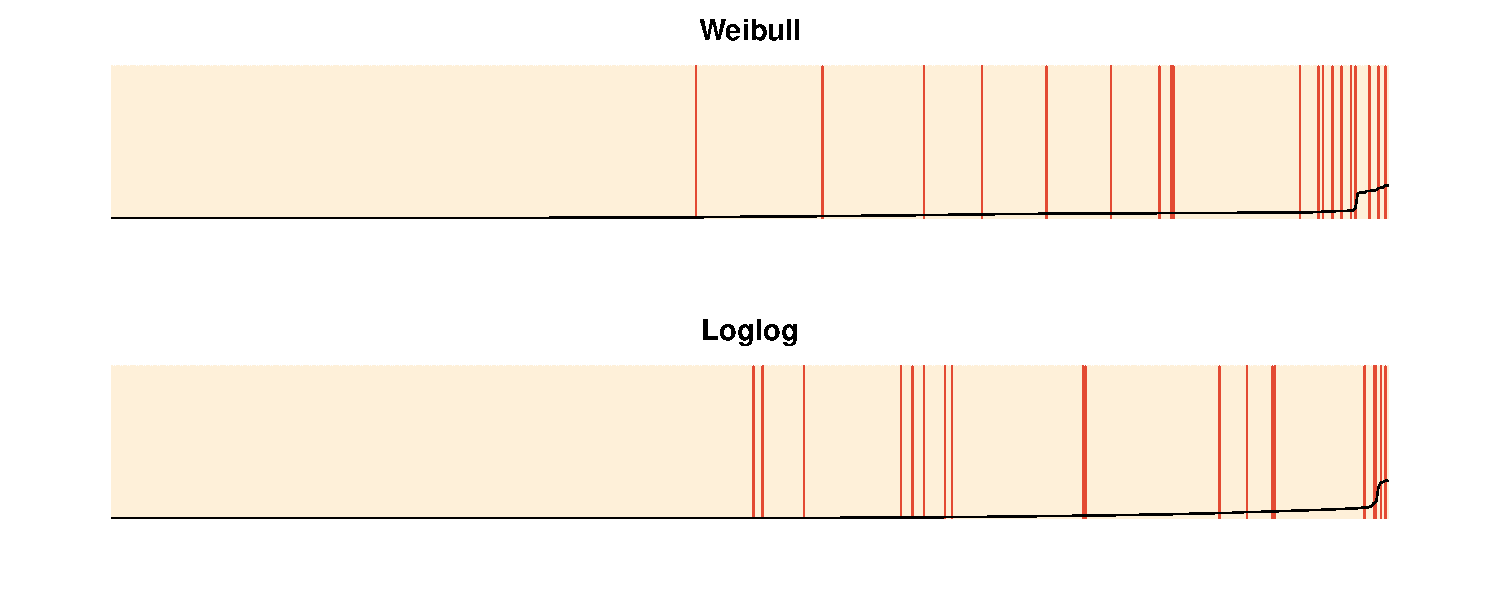
\includegraphics[width=0.8\textwidth]{graphics/oos-sepplots.pdf}
\caption{Out-of-sample separation plots.}
\label{oos-sepplots}
\end{center}
\end{figure}

\section{Additional discussion}

\subsection{Censoring considerations}

Truncation and censoring are problematic for split-population duration
models, as they are for standard duration regression, but also pose some
additional considerations. In left-truncation, we do not observe data
for a spell prior to some date, and thus have incomplete and inaccurate
values for the duration or time to failure for a spell. Since immune
spells in the sample are over time going to distinguish themselves with
exceptionally long survival times compared to spells at risk which fail
periodically, left-censoring also makes it more difficult to distinguish
the immune and at risk subpopulations.

Sometimes information about previous failures in the data is available
beyond the time period over which covariates are observed, making it
possible to ameliorate or eliminate left-censoring by using the
information of previous failures when constructing the necessary
duration variables with \code{add\_duration()}.

Right-censoring, where spells end before outcomes are observed, also
pose a unique problem in the split-population framework. Although
right-censored spells themselves are accommodated in the modeling
function, they impact the coding of at risk vs.~immune spells. The
\code{add\_duration()} function retroactively codes all observations in
a spell as at risk if the spell itself ended in failure. Right-censored
spells are coded as immune over their entire duration. This can lead to
some misclassification of observations as immune even though they
experience failure at some point in the unobserved future.

Furthermore, as the example above shows, in out-of-sample testing based
on some kind of data partitioning scheme, this coding scheme can lead to
unintentional contamination of in-sample cases with knowledge of
out-of-sample failures through the risk coding for failed spells. This
leads to two recommendations. First, data should be partitioned spell or
block-wise, e.g., by withholding the last \emph{x} years of data, and
not randomly. Second, given the two concerns of left-censoring and
non-independence induced through the duration and risk coding, care
should be taken to ensure that duration data are built without access to
future information in another data partition.

\subsection{Comparison with other software}

The \CRANpkg{survival} library \citep{thernau2000modeling, thernau2015survival}, arguably the most well-established library for survival and event history analysis in {\sf R}, allows for the estimation of a wide variety of semi-, non-, and parametric survival models, and provides facilities for handling and descriptive summaries of survival and event history data. It does not include cure rate or split-population mixture models of the type we have implemented though.

One useful extension of our project in the future would be to integrate and adapt the \code{Surv} class for survival data in \CRANpkg{survival} to the \CRANpkg{spduration} library. This would require some modification of the class as our model also requires information on the risk status of spells, but would give access to the much broader functionality, especially for descriptive summaries of data, in the \CRANpkg{survival} library. 

Other currently available {\sf R} routines for estimation of split-population/cure rate duration models include the packages \CRANpkg{smcure}  \citep{cai2012smcureR}, described in \citet{cai2012smcure}, and \pkg{nltm} \citep{garibotti2010nltm}. \CRANpkg{smcure} implements semi-parametric proportional hazards and accelerated failure time cure models using estimation procedures presented in \citet{peng2003fitting} and \citet{zhang2007new}.\footnote{There is also the older \pkg{gfcure} package, which estimates the parametric accelerated failure time cure model discussed in \citet{peng1998generalized}. A version for Windows is available at \url{http://post.queensu.ca/~pengp/software.html}.} The package \pkg{nltm} will estimate a semi-parametric proportional hazard cure model, and a number of other survival models, using the approach developed in \citet{tsodikov2003semiparametric,tsodikov2007profile}. Semi-parametric estimation of the hazard function is attractive because it requires no assumption about its shape, and such assumptions can be difficult in practice to empirically evaluate. The main advantage \CRANpkg{spduration} offers is the ability to include time varying covariates, which gives it a broader range of practical applications, as \CRANpkg{smcure} and \pkg{nltm} will only accommodate case-based data. \CRANpkg{spduration} also features more post-estimation methods than alternative packages, including those discussed above to create and evaluate model predictions.  

%Finally, there are {\sf Stata} routines for implementing cure models \citep[see, e.g.,][]{lambert2007modeling,buxton2013cureregr}, some of which can handle time-varying covariates, but this is of course of limited appeal to {\sf R} users. 

\section{Conclusion}

\begin{figure}[htbp!]
\centering
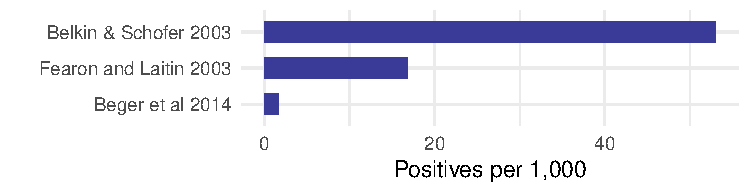
\includegraphics[width = 4in]{graphics/rates.pdf}
\caption{Rates of positive outcomes in select publications with binary outcomes.}
\label{rates}
\end{figure}

Many outcomes of interest are rare events. For example, coups, war
onset, or mass killings are exceedingly rare events when considering
that most countries do not experience high levels of violence. Figure
\ref{rates} shows a few examples of published research that models
binary outcomes. \citet{fearon2003ethnicity} is a widely cited study of
civil war onset that uses yearly observations of all major countries;
\citet{beger2014ensemble} is an example of the positive rates when
moving to monthly data for a similar set of countries. The positive
rates range from 5 to less than 0.2\% of all data points.\footnote{For a
  discussion of the difficulties rare events can pose for prediction see
  \citet{king2001explaining} and \citet{king2001logistic}.}

In the language of machine learning, we are dealing with highly
imbalanced classes. It is a well-recognized problem and has led to the
development or use of several specialized mixture models like
zero-inflated Poisson and negative binomial regression for count data,
and a zero-inflated ordered probit for ordinal outcomes \citep{bagozzi2015modeling}. Split-population duration regression provides another principled
solution to the challenges posed by data in this domain, but, unlike
other solutions to the sparse outcome problem, also addresses underlying
temporal dynamics that are an important part of the non-independent data
political scientists and other social scientists commonly use.

Split-population duration models are not only appealing in a technical
sense, but they also match the logic or intuition many social scientists
use when they distinguish long-term risk factors from more fleeting
triggering causes. The example we have used, \citet{belkin2003toward},
is a particularly clear illustration of how well the language of
theorists maps onto the model intuition.

\bibliography{beger-hill-metternich-minhas-ward}

\address{Andreas Beger\\
  Ward Associates\\
  Tallinn\\
  Estonia\\
  \email{adbeger@gmail.com}}

\address{Daniel W. Hill, Jr.\\
  Department of International Affairs\\
  School of Public and International Affairs, University of Georgia\\
  Candler Hall, Athens GA 30602\\
  United States of America\\
  \email{dwhill@uga.edu}}

\address{Nils W. Metternich\\
  Department of Political Science\\
University College London\\
  London\\
  United Kingdom\\
  \email{n.metternich@ucl.ac.uk}\\
  Nils W. Metternich acknowledges support from the Economic and Social Research Council (ES/L011506/1)}
  

\address{Shahryar Minhas\\
  Department of Political Science\\
  Duke University\\
  Durham, NC\\
  United States of America\\
  \email{sfm12@duke.edu}}

\address{Michael D. Ward\\
  Department of Political Science\\
  Duke University\\
  Durham, NC\\
  United States of America\\
  \email{michael.d.ward@duke.edu}}
